%
%    This program is free software; you can redistribute it and/or modify
%    it under the terms of the GNU General Public License as published by
%    the Free Software Foundation; either version 2 of the License, or
%    (at your option) any later version.
%
%    This program is distributed in the hope that it will be useful,
%    but WITHOUT ANY WARRANTY; without even the implied warranty of
%    MERCHANTABILITY or FITNESS FOR A PARTICULAR PURPOSE.  See the
%    GNU General Public License for more details.
%
%    You should have received a copy of the GNU General Public License
%    along with this program; if not, write to the Free Software
%    Foundation, Inc., 675 Mass Ave, Cambridge, MA 02139, USA.
%

% Version: $Revision$

The plugin architecture of the Explorer allows you to add new functionality
easily without having to dig into the code of the Explorer itself. In the
following you will find information on how to add new tabs, like the
``Classify'' tab, and new visualization plugins for the ``Classify'' tab.

\subsection{Adding tabs}
The Explorer is a handy tool for initial exploration of your data -- for
proper statistical evaluation, the Experimenter should be used instead. But if
the available functionality is not enough, you can always add your own
custom-made tabs to the Explorer.

\subsubsection{Requirements}
Here is roughly what is required in order to add a new tab (the examples below
go into more detail):
\begin{tight_itemize}
  \item your class must be derived from \texttt{javax.swing.JPanel}
  \item the interface \texttt{weka.gui.explorer.Explorer.ExplorerPanel} must be
implemented by your class
  \item optional interfaces
  \begin{tight_itemize}
	\item \texttt{weka.gui.explorer.Explorer.LogHandler} -- in case
you want to take advantage of the logging in the Explorer
	\item \texttt{weka.gui.explorer.Explorer.CapabilitiesFilterChangeListener}
-- in case your class needs to be notified of changes in the
Capabilities, e.g., if new data is loaded into the Explorer
  \end{tight_itemize}
  \item adding the classname of your class to the Tabs property in the
\texttt{Explorer.props} file
\end{tight_itemize}

\subsubsection{Examples}
The following examples demonstrate the plugin architecture. Only the
necessary details are discussed, as the full source code is available from the
WEKA Examples \cite{wekaexamples} (package \texttt{wekaexamples.gui.explorer}).

\subsubsection*{SQL worksheet}
\subsubsection*{Purpose}
Displaying the SqlViewer as a tab in the Explorer instead of using it either via
the \textit{Open DB...} button or as standalone application. Uses the existing
components already available in WEKA and just assembles them in a
\texttt{JPanel}. Since this tab does not rely on a dataset being loaded into the
Explorer, it will be used as a \textit{standalone} one.

Useful for people who are working a lot with databases and would like to have an
SQL worksheet available all the time instead of clicking on a button every time
to open up a database dialog.

\subsubsection*{Implementation}
\begin{tight_itemize}
  \item class is derived from \texttt{javax.swing.JPanel} and implements the
interface \texttt{weka.gui.Explorer.ExplorerPanel} (the full source code also
imports the \texttt{weka.gui.Explorer.LogHandler} interface, but that is only
additional functionality):
  \begin{verbatim}
  public class SqlPanel
    extends JPanel
    implements ExplorerPanel {
  \end{verbatim}

  \item some basic members that we need to have
  \begin{verbatim}
  /** the parent frame */
  protected Explorer m_Explorer = null;

  /** sends notifications when the set of working instances gets changed*/
  protected PropertyChangeSupport m_Support = new PropertyChangeSupport(this);
  \end{verbatim}

  \item methods we need to implement due to the used interfaces
  \begin{verbatim}
  /** Sets the Explorer to use as parent frame */
  public void setExplorer(Explorer parent) {
    m_Explorer = parent;
  }

  /** returns the parent Explorer frame */
  public Explorer getExplorer() {
    return m_Explorer;
  }

  /** Returns the title for the tab in the Explorer */
  public String getTabTitle() {
    return "SQL";  // what's displayed as tab-title, e.g., Classify
  }

  /** Returns the tooltip for the tab in the Explorer */
  public String getTabTitleToolTip() {
    return "Retrieving data from databases";  // the tooltip of the tab
  }

  /** ignored, since we "generate" data and not receive it */
  public void setInstances(Instances inst) {
  }

  /** PropertyChangeListener which will be notified of value changes. */
  public void addPropertyChangeListener(PropertyChangeListener l) {
    m_Support.addPropertyChangeListener(l);
  }

  /** Removes a PropertyChangeListener. */
  public void removePropertyChangeListener(PropertyChangeListener l) {
    m_Support.removePropertyChangeListener(l);
  }
  \end{verbatim}

  \newpage
  \item additional GUI elements
  \begin{verbatim}
  /** the actual SQL worksheet */
  protected SqlViewer m_Viewer;

  /** the panel for the buttons */
  protected JPanel m_PanelButtons;

  /** the Load button - makes the data available in the Explorer */
  protected JButton m_ButtonLoad = new JButton("Load data");

  /** displays the current query */
  protected JLabel m_LabelQuery = new JLabel("");
  \end{verbatim}

  \item loading the data into the Explorer by clicking on the \textit{Load}
button will fire a \textit{propertyChange} event:
  \begin{verbatim}
    m_ButtonLoad.addActionListener(new ActionListener() {
      public void actionPerformed(ActionEvent evt){
        m_Support.firePropertyChange("", null, null);
      }
    });
  \end{verbatim}

  \item the \textit{propertyChange} event will perform the actual loading of the
data, hence we add an anonymous property change listener to our panel:
  \begin{verbatim}
  addPropertyChangeListener(new PropertyChangeListener() {
    public void propertyChange(PropertyChangeEvent e) {
      try {
        // load data
        InstanceQuery query = new InstanceQuery();
        query.setDatabaseURL(m_Viewer.getURL());
        query.setUsername(m_Viewer.getUser());
        query.setPassword(m_Viewer.getPassword());
        Instances data = query.retrieveInstances(m_Viewer.getQuery());

        // set data in preprocess panel (also notifies of capabilties changes)
        getExplorer().getPreprocessPanel().setInstances(data);
      }
      catch (Exception ex) {
        ex.printStackTrace();
      }
    }
  });
  \end{verbatim}

  \item In order to add our \texttt{SqlPanel} to the list of tabs displayed in
the Explorer, we need to modify the \texttt{Explorer.props} file (just extract
it from the \texttt{weka.jar} and place it in your home directory). The
\texttt{Tabs} property must look like this:
  \begin{verbatim}
  Tabs=weka.gui.explorer.SqlPanel,\
       weka.gui.explorer.ClassifierPanel,\
       weka.gui.explorer.ClustererPanel,\
       weka.gui.explorer.AssociationsPanel,\
       weka.gui.explorer.AttributeSelectionPanel,\
       weka.gui.explorer.VisualizePanel
  \end{verbatim}
\end{tight_itemize}

\newpage
\subsubsection*{Screenshot}
\begin{center}
	\epsfig{file=images/extending/SqlPanel.eps,width=12cm}
\end{center}

\newpage
\subsubsection*{Artificial data generation}
\subsubsection*{Purpose}
Instead of only having a \textit{Generate...} button in the PreprocessPanel or
using it from command-line, this example creates a new panel to be displayed as
extra tab in the Explorer. This tab will be available regardless whether a
dataset is already loaded or not (= standalone).

\subsubsection*{Implementation}
\begin{tight_itemize}
  \item class is derived from \texttt{javax.swing.JPanel} and implements the
interface \texttt{weka.gui.Explorer.ExplorerPanel} (the full source code also
imports the \texttt{weka.gui.Explorer.LogHandler} interface, but that is only
additional functionality):
  \begin{verbatim}
  public class GeneratorPanel
    extends JPanel
    implements ExplorerPanel {
  \end{verbatim}

  \item some basic members that we need to have (the same as for the
\texttt{SqlPanel} class):
  \begin{verbatim}
  /** the parent frame */
  protected Explorer m_Explorer = null;

  /** sends notifications when the set of working instances gets changed*/
  protected PropertyChangeSupport m_Support = new PropertyChangeSupport(this);
  \end{verbatim}

  \item methods we need to implement due to the used interfaces (almost
identical to \texttt{SqlPanel}):
  \begin{verbatim}
  /** Sets the Explorer to use as parent frame */
  public void setExplorer(Explorer parent) {
    m_Explorer = parent;
  }
  /** returns the parent Explorer frame */
  public Explorer getExplorer() {
    return m_Explorer;
  }
  /** Returns the title for the tab in the Explorer */
  public String getTabTitle() {
    return "DataGeneration";  // what's displayed as tab-title, e.g., Classify
  }
  /** Returns the tooltip for the tab in the Explorer */
  public String getTabTitleToolTip() {
    return "Generating artificial datasets";  // the tooltip of the tab
  }
  /** ignored, since we "generate" data and not receive it */
  public void setInstances(Instances inst) {
  }
  /** PropertyChangeListener which will be notified of value changes. */
  public void addPropertyChangeListener(PropertyChangeListener l) {
    m_Support.addPropertyChangeListener(l);
  }
  /** Removes a PropertyChangeListener. */
  public void removePropertyChangeListener(PropertyChangeListener l) {
    m_Support.removePropertyChangeListener(l);
  }
  \end{verbatim}

  \newpage
  \item additional GUI elements:
  \begin{verbatim}
  /** the GOE for the generators */
  protected GenericObjectEditor m_GeneratorEditor = new GenericObjectEditor();

  /** the text area for the output of the generated data */
  protected JTextArea m_Output = new JTextArea();

  /** the Generate button */
  protected JButton m_ButtonGenerate = new JButton("Generate");

  /** the Use button */
  protected JButton m_ButtonUse = new JButton("Use");
  \end{verbatim}

  \item the \textit{Generate} button does not load the generated data directly
into the Explorer, but only outputs it in the \texttt{JTextArea} (the
\textit{Use} button loads the data - see further down):
  \begin{verbatim}
  m_ButtonGenerate.addActionListener(new ActionListener(){
    public void actionPerformed(ActionEvent evt){
      DataGenerator generator = (DataGenerator) m_GeneratorEditor.getValue();
      String relName = generator.getRelationName();

      String cname = generator.getClass().getName().replaceAll(".*\\.", "");
      String cmd = generator.getClass().getName();
      if (generator instanceof OptionHandler)
        cmd += " "+Utils.joinOptions(((OptionHandler)generator).getOptions());

      try {
        // generate data
        StringWriter output = new StringWriter();
        generator.setOutput(new PrintWriter(output));
        DataGenerator.makeData(generator, generator.getOptions());
        m_Output.setText(output.toString());
      }
      catch (Exception ex) {
        ex.printStackTrace();
        JOptionPane.showMessageDialog(
          getExplorer(), "Error generating data:\n" + ex.getMessage(),
          "Error", JOptionPane.ERROR_MESSAGE);
      }

      generator.setRelationName(relName);
    }
  });
  \end{verbatim}

  \item the \textit{Use} button finally fires a \textit{propertyChange} event
that will load the data into the Explorer:
  \begin{verbatim}
    m_ButtonUse.addActionListener(new ActionListener(){
      public void actionPerformed(ActionEvent evt){
        m_Support.firePropertyChange("", null, null);
      }
    });
  \end{verbatim}

  \newpage
  \item the \textit{propertyChange} event will perform the actual loading of the
data, hence we add an anonymous property change listener to our panel:
  \begin{verbatim}
  addPropertyChangeListener(new PropertyChangeListener() {
    public void propertyChange(PropertyChangeEvent e) {
      try {
        Instances data = new Instances(new StringReader(m_Output.getText()));
        // set data in preprocess panel (also notifies of capabilties changes)
        getExplorer().getPreprocessPanel().setInstances(data);
      }
      catch (Exception ex) {
        ex.printStackTrace();
        JOptionPane.showMessageDialog(
          getExplorer(), "Error generating data:\n" + ex.getMessage(),
          "Error", JOptionPane.ERROR_MESSAGE);
      }
    }
  });
  \end{verbatim}

  \item In order to add our \texttt{GeneratorPanel} to the list of tabs
displayed in the Explorer, we need to modify the \texttt{Explorer.props} file
(just extract it from the \texttt{weka.jar} and place it in your home
directory). The \texttt{Tabs} property must look like this:
  \begin{verbatim}
  Tabs=weka.gui.explorer.GeneratorPanel:standalone,\
       weka.gui.explorer.ClassifierPanel,\
       weka.gui.explorer.ClustererPanel,\
       weka.gui.explorer.AssociationsPanel,\
       weka.gui.explorer.AttributeSelectionPanel,\
       weka.gui.explorer.VisualizePanel
  \end{verbatim}

\item \textbf{Note:} the standalone option is used to make the tab available
without requiring the preprocess panel to load a dataset first.
\end{tight_itemize}

\subsubsection*{Screenshot}
\begin{center}
	\epsfig{file=images/extending/GeneratorPanel.eps,width=12cm}
\end{center}

\newpage
\subsubsection*{Experimenter "light"}
\subsubsection*{Purpose}
By default the Classify panel only performs 1 run of 10-fold cross-validation.
Since most classifiers are rather sensitive to the order of the data being
presented to them, those results can be too optimistic or pessimistic. Averaging
the results over 10 runs with differently randomized train/test pairs returns
more reliable results. And this is where this plugin comes in: it can be used to
obtain statistical sound results for a specific classifier/dataset combination,
without having to setup a whole experiment in the Experimenter.

\subsubsection*{Implementation}
\begin{tight_itemize}
  \item Since this plugin is rather bulky, we omit the implementation details,
but the following can be said:
  \begin{tight_itemize}
	\item based on the \texttt{weka.gui.explorer.ClassifierPanel}
	\item the actual code doing the work follows the example in the
\textit{Using the Experiment API} wiki article \cite{wekawiki}
  \end{tight_itemize}
  \item In order to add our \texttt{ExperimentPanel} to the list of tabs
displayed in the Explorer, we need to modify the \texttt{Explorer.props} file
(just extract it from the \texttt{weka.jar} and place it in your home
directory). The \texttt{Tabs} property must look like this:
  \begin{verbatim}
  Tabs=weka.gui.explorer.ClassifierPanel,\
       weka.gui.explorer.ExperimentPanel,\
       weka.gui.explorer.ClustererPanel,\
       weka.gui.explorer.AssociationsPanel,\
       weka.gui.explorer.AttributeSelectionPanel,\
       weka.gui.explorer.VisualizePanel
  \end{verbatim}
\end{tight_itemize}

\subsubsection*{Screenshot}
\begin{center}
	\epsfig{file=images/extending/ExperimentPanel.eps,width=12cm}
\end{center}

\newpage
\subsection{Adding visualization plugins}
\subsubsection{Introduction}
You can add visualization plugins in the Explorer (Classify panel). This
makes it easy to implement custom visualizations, if the ones WEKA offers are
not sufficient. The following examples can be found in the Examples collection
\cite{wekaexamples} (package \texttt{wekaexamples.gui.visualize.plugins}).
The following types of plugins are available and explained in the sections
below:
\begin{tight_itemize}
  \item predictions -- for displaying the predictions
  \item errors -- for plotting actual vs predicted
  \item graphs -- for displaying graphs generated by \texttt{BayesNet}
  \item trees -- for displaying trees generated by classifiers like \texttt{J48}
\end{tight_itemize}

%%%%%%%%%%%%%%%
% Predictions %
%%%%%%%%%%%%%%%

\subsubsection{Predictions}
\label{visualization_predictions}
\heading{Requirements}
\begin{tight_itemize}
  \item custom visualization class must implement the following interface
  \begin{verbatim}
  weka.gui.visualize.plugins.VisualizePlugin
  \end{verbatim}
  
  \item the class must either reside in the following package (visualization
classes are automatically discovered during run-time)
  \begin{verbatim}
  weka.gui.visualize.plugins
  \end{verbatim}
  
  \item or you must list the package this class belongs to in the properties
file \texttt{weka/gui/GenericPropertiesCreator.props} (or the equivalent in
your home directory) under the key
\texttt{weka.gui.visualize.plugins.VisualizePlugin}.
\end{tight_itemize}

\heading{Implementation}
The visualization interface contains the following four methods
\begin{tight_itemize}
  \item \texttt{getMinVersion} -- This method returns the minimum version
(inclusive) of WEKA that is necessary to execute the plugin, e.g., 3.5.0.
  \item \texttt{getMaxVersion} -- This method returns the maximum version
(exclusive) of WEKA that is necessary to execute the plugin, e.g., 3.6.0.
  \item \texttt{getDesignVersion} -- Returns the actual version of WEKA
this plugin was designed for, e.g., 3.5.1
  \item \texttt{getVisualizeMenuItem} -- The \texttt{JMenuItem} that is returned
via this method will be added to the plugins menu in the popup in the Explorer.
The \texttt{ActionListener} for clicking the menu item will most likely open a
new frame containing the visualized data.
\end{tight_itemize}

\newpage
\heading{Examples}
\heading{Table with predictions}
The \texttt{PredictionTable.java} example simply displays the actual class label
and the one predicted by the classifier. In addition to that, it lists whether
it was an incorrect prediction and the class probability for the correct class
label.
\begin{center}
	\epsfig{file=images/extending/PredictionTable.eps,width=12cm}
\end{center}

\newpage
\heading{Bar plot with probabilities}
The \texttt{PredictionError.java} example uses the JMathTools library (needs
the \texttt{jmathplot.jar} \cite{jmathplot} in the CLASSPATH) to display a
simple bar plot of the
predictions. The correct predictions are displayed in blue, the incorrect ones
in red. In both cases the class probability that the classifier returned for the
correct class label is displayed on the y axis. The x axis is simply the index
of the prediction starting with 0.
\begin{center}
	\epsfig{file=images/extending/PredictionError.eps,width=12cm}
\end{center}

%%%%%%%%%%
% Errors %
%%%%%%%%%%

\newpage
\subsubsection{Errors}
\heading{Requirements}
Almost the same requirements as for the visualization of the predictions (see
section \ref{visualization_predictions}), but with the following differences:
\begin{tight_itemize}
  \item \texttt{weka.gui.visualize.plugins.ErrorVisualizePlugin} -- is the
interface to implement
  \item \texttt{weka.gui.visualize.plugins.ErrorVisualizePlugin} -- is the key
in the \texttt{GenericPropertiesCreator.props} file to list the package name 
\end{tight_itemize}

\heading{Examples}
\texttt{weka.classifiers.functions.LinearRegression} was used to generate the
following screenshots using default parameters on the UCI dataset
\textit{bolts}, using a percentage split of 66\% for the training set and the
remainder for testing.

\heading{Using WEKA panels}
The \texttt{ClassifierErrorsWeka.java} example simply displays the classifier
errors like the \textit{Visualize classifier errors} menu item already available
in WEKA. It is just to demonstrate how to use existing WEKA classes.

\begin{center}
    \epsfig{file=images/extending/ClassifierErrorsWeka.eps,width=12cm}
\end{center}

\newpage
\heading{Using JMathtools' Boxplot }
The \texttt{ClassifierErrorsMathtools.java} example uses the JMathTools library
(needs the \texttt{jmathplot.jar} \cite{jmathplot} in the CLASSPATH) to display
a boxplot (the width of the boxes is 0, to make it look like an error plot). The
relative error per prediction is displayed as vertical line.
\begin{center}
    \epsfig{file=images/extending/ClassifierErrorsMathtools.eps,width=12cm}
\end{center}
\textbf{Note:} This display is only available for \textit{numeric} classes.

%%%%%%%%%%
% Graphs %
%%%%%%%%%%

\newpage
\subsubsection{Graphs}
\heading{Requirements}
Almost the same requirements as for the visualization of the predictions (see
section \ref{visualization_predictions}), but with the following differences:
\begin{tight_itemize}
  \item \texttt{weka.gui.visualize.plugins.GraphVisualizePlugin} -- is the
interface to implement
  \item \texttt{weka.gui.visualize.plugins.GraphVisualizePlugin} -- is the key
in the \texttt{GenericPropertiesCreator.props} file to list the package name
\end{tight_itemize}

\heading{Examples}
\heading{prefuse visualization toolkit}
The \texttt{PrefuseGraph.java} example uses the \textit{prefuse visualization
toolkit} (prefuse-beta, 2007.10.21 \cite{prefuse}). It is based on the
\texttt{prefuse.demos.GraphView} demo class.

The following screenshot was generated using \texttt{BayesNet} on the UCI
dataset \textit{anneal} with the following parametrization:
\begin{verbatim}
  weka.classifiers.bayes.BayesNet -D -Q
    weka.classifiers.bayes.net.search.local.K2 -- -P 3 -S BAYES -E
    weka.classifiers.bayes.net.estimate.SimpleEstimator -- -A 0.5
\end{verbatim}
\begin{center}
    \epsfig{file=images/extending/PrefuseGraph.eps,width=12cm}
\end{center}

%%%%%%%%%
% Trees %
%%%%%%%%%

\newpage
\subsubsection{Trees}
\heading{Requirements}
Almost the same requirements as for the visualization of the predictions (see
section \ref{visualization_predictions}), but with the following differences:
\begin{tight_itemize}
  \item \texttt{weka.gui.visualize.plugins.TreeVisualizePlugin} -- is the
interface to implement
  \item \texttt{weka.gui.visualize.plugins.TreeVisualizePlugin} -- is the key
in the \texttt{GenericPropertiesCreator.props} file to list the package name
\end{tight_itemize}

\heading{Examples}
\heading{prefuse visualization toolkit}
The \texttt{PrefuseTree.java} example uses the \textit{prefuse visualization
toolkit} (prefuse-beta, 2007.10.21 \cite{prefuse}). It is based on the
\texttt{prefuse.demos.TreeView} demo class.

The following screenshot was generated using \texttt{J48} on the UCI dataset
\textit{anneal} with default parameters:
\begin{center}
    \epsfig{file=images/extending/PrefuseTreeClassifier.eps,width=12cm}
\end{center}

\newpage
And here is an example of \texttt{Cobweb} on the same dataset, once again with
default parameters:
\begin{center}
    \epsfig{file=images/extending/PrefuseTreeClusterer.eps,width=12cm}
\end{center}
